\chapter{La régulation de la pression artérielle et l'exercice}\label{ch:b2:blood-pressure}

Levez-vous brusquement après être resté allongé et, pendant une
seconde, un demi-litre de \omterm{def:b2:blood-circulation:blood}{sang} s'accumule dans les \omterm{def:b2:blood-circulation:vessels}{veines} des jambes~;
le \omterm{def:b2:heart:anatomy}{cœur}, recevant moins, pompe moins, la pression au niveau de la tête
chute, et le cerveau --- qui se trouve à \qty{40}{cm} au-dessus du \omterm{def:b2:heart:anatomy}{cœur} et
ne peut pas stocker de dioxygène --- est à une seconde ou deux de la
syncope. Il ne défaille presque jamais, parce qu'en un battement un
réflexe a resserré les \omterm{def:b2:blood-circulation:vessels}{artérioles} et accéléré le \omterm{def:b2:heart:anatomy}{cœur}. Courez pour
attraper un bus, et les muscles ont besoin de dix fois plus de \omterm{def:b2:blood-circulation:blood}{sang}
qu'au repos~; ils l'obtiennent en une minute, et la pression qui le
propulse reste stable alors que la résistance du corps entier diminue
des deux tiers. Ce chapitre traite de cette régulation~: ce qui fixe la
pression, comment elle est perçue, le réflexe rapide et les hormones
lentes qui la corrigent, et la manière dont l'exercice réorganise le
système au lieu de le court-circuiter.

\section{Ce qu'est la pression}

\begin{theorem}[L'équation de la circulation]\label{thm:b2:blood-pressure:equation}
\index{pression arterielle moyenne@pression artérielle moyenne}\index{resistance peripherique totale@résistance périphérique totale}
La \omterm{thm:b2:blood-pressure:equation}{pression artérielle moyenne} $\bar P$ est le produit de ce que le \omterm{def:b2:heart:anatomy}{cœur}
fait entrer par ce que les vaisseaux laissent sortir~:
\[
\bar P - P_{\text{ven}} = Q\,R, \qquad Q = f\times V_s,
\]
où $Q$ est le \omterm{thm:b2:heart:starling}{débit cardiaque} (fréquence cardiaque $f$ multipliée par le
volume d'éjection
$V_s$), $R$ la \omterm{thm:b2:blood-pressure:equation}{résistance périphérique totale} --- les \omterm{def:b2:blood-circulation:vessels}{artérioles} de tous
les organes en parallèle --- et $P_{\text{ven}}$ la pression veineuse,
voisine de zéro. Au repos, $\qty{5}{L/min}\times\qty{1.08}{mmHg.s/mL}$
donne \qty{90}{mmHg}. Toute régulation de la pression agit sur l'une de
trois grandeurs~: la fréquence, le volume d'éjection (par le remplissage
et la contractilité du \cref{ch:b2:heart}) ou la résistance (par le
rayon artériolaire, à la puissance quatre). Comme les organes sont en
parallèle, le débit de chacun est sa part de la pression divisée par sa
propre résistance~: dilater les \omterm{def:b2:blood-circulation:vessels}{artérioles} d'un organe augmente son
débit sans modifier celui des autres, à condition que la pression soit
maintenue --- et maintenir la pression est précisément le rôle de la
régulation.
\end{theorem}
\begin{proof}
Loi d'Ohm pour un fluide~: le débit à travers une résistance est la
chute de pression à ses bornes divisée par la résistance (Poiseuille,
\cref{ch:b2:blood-circulation})~; pour des résistances en parallèle, les
débits s'ajoutent et $1/R = \sum 1/R_i$. La pression moyenne sur un
battement vaut approximativement la pression diastolique plus un tiers
de la \omterm{thm:b2:blood-circulation:windkessel}{pression différentielle}~:
$80 + 40/3 = \qty{93}{mmHg}$.
\end{proof}

\begin{omfigure}
\begin{tikzpicture}[every node/.style={font=\scriptsize}, >=stealth]
  \node[draw, rounded corners, fill=omThm!15, minimum width=2.4cm, minimum height=1cm, align=center] (heart) at (0,0) {cœur\\$Q = f\,V_s$};
  \draw[very thick, omThm] (1.2,0) -- (2.4,0);
  \draw[very thick, omThm] (2.4,-2.4) -- (2.4,2.4);
  \foreach \y/\org/\r in {2.0/{cerveau}/{$R_1$}, 1.0/{muscle cardiaque}/{$R_2$}, 0/{intestin et foie}/{$R_3$}, -1.0/{reins}/{$R_4$}, -2.0/{muscles, peau}/{$R_5$}} {
    \draw[very thick, omThm] (2.4,\y) -- (3.6,\y);
    \draw[thick, decorate, decoration={zigzag, segment length=4pt, amplitude=2pt}] (3.6,\y) -- (5.0,\y);
    \node[above] at (4.3,\y+0.05) {\org};
    \node[below] at (4.3,\y-0.05) {\r};
    \draw[very thick, omDef] (5.0,\y) -- (6.2,\y);
  }
  \draw[very thick, omDef] (6.2,-2.4) -- (6.2,2.4);
  \draw[very thick, omDef] (6.2,0) -- (7.4,0) |- (0,-3.2) -- (0,-0.5);
  \node[omThm, above] at (1.8,0.05) {$\bar P$};
  \node[omDef, below] at (3.7,-3.2) {veines, $P_{\text{ven}} \approx 0$};
  \node[anchor=west, align=left] at (7.8,1.5) {organes en parallèle~:\\$1/R = \sum 1/R_i$\\débit vers l'organe $i$~: $\bar P/R_i$};
\end{tikzpicture}

{\small La circulation vue comme un circuit~: une pompe, une pression, et
les résistances artériolaires des organes en parallèle. Chaque organe
reçoit $\bar P/R_i$~; la régulation maintient $\bar P$ tandis que les
$R_i$ s'ajustent à la demande.}
\end{omfigure}

\begin{proposition}[Pourquoi la pression doit être régulée]\label{prop:b2:blood-pressure:why}
Trop basse, et le cerveau --- situé à \qty{40}{cm} au-dessus du \omterm{def:b2:heart:anatomy}{cœur} chez un
adulte debout, ce qui coûte \qty{31}{mmHg} de charge hydrostatique ---
ainsi que le muscle cardiaque lui-même sont insuffisamment irrigués~: le
cerveau défaille en quelques secondes. Trop haute, et les vaisseaux sont
endommagés~: la paroi artérielle s'épaissit et se rigidifie, les
glomérules du rein se cicatrisent, la rétine saigne, et le \omterm{def:b2:heart:anatomy}{cœur} peine
contre la pression jusqu'à défaillir. La pression doit aussi rester
stable tandis que les besoins des organes varient d'un ordre de grandeur
--- l'intestin après un repas, les muscles à l'effort, la peau par forte
chaleur --- et tandis que le volume sanguin lui-même est perdu par
hémorragie ou par la sueur. Deux systèmes s'en chargent~: un réflexe
nerveux qui agit en un battement sur la fréquence, le volume d'éjection
et la résistance, et des systèmes hormonaux qui agissent sur des heures
et des jours sur la résistance et, surtout, sur le volume sanguin par
l'intermédiaire du rein.
\end{proposition}

\begin{omfigure}
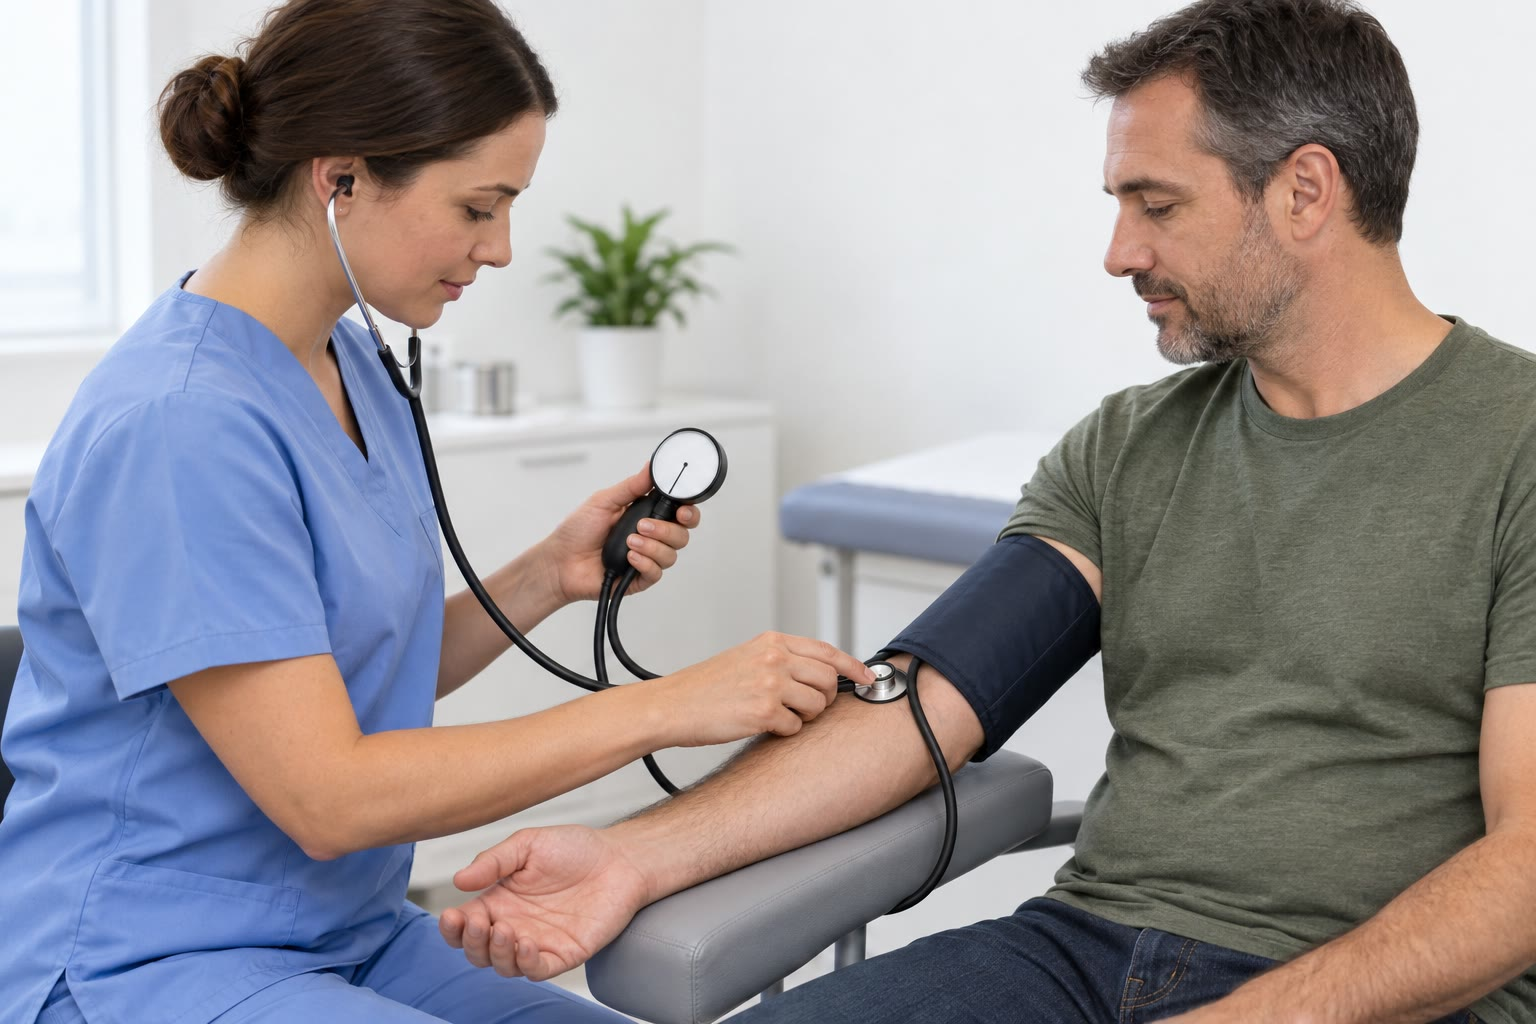
\includegraphics[width=0.6\linewidth]{images/book4/ai/b4-18-blood-pressure-cuff.jpg}

{\small La mesure de la pression. Le brassard est gonflé au-dessus de la
pression systolique, si bien qu'aucun \omterm{def:b2:blood-circulation:blood}{sang} ne passe~; lorsqu'on le
dégonfle, les premiers bruits d'écoulement turbulent perçus au
stéthoscope marquent la pression systolique, et leur disparition,
lorsque l'\omterm{def:b2:blood-circulation:vessels}{artère} reste ouverte pendant tout le cycle, marque la
diastolique.}
\end{omfigure}

\section{La boucle rapide~: le baroréflexe}

\begin{definition}[Le baroréflexe]\label{def:b2:blood-pressure:baroreflex}
\index{barorecepteur@barorécepteur}\index{baroreflexe@baroréflexe}\index{centre vasomoteur}\index{systeme nerveux autonome@système nerveux autonome}
Des récepteurs d'étirement situés dans la paroi des sinus carotidiens (à
la bifurcation de chaque \omterm{def:b2:blood-circulation:vessels}{artère} carotide, sous la mâchoire) et de la
crosse aortique --- les \emph{barorécepteurs} --- émettent des influx à
une fréquence qui augmente avec la pression qui les distend, et plus
vite encore lorsque la pression monte. Leurs nerfs rejoignent les
\emph{centres cardiovasculaires} du bulbe rachidien, qui commandent les
deux branches de la sortie autonome~: le \omterm{prop:b2:heart:control}{nerf vague}, dont l'acétylcholine
ralentit le \omterm{prop:b2:heart:conduction}{nœud sinusal}, et les nerfs sympathiques, dont la
noradrénaline accélère le nœud, renforce le \omterm{def:b2:heart:anatomy}{ventricule}, contracte les
\omterm{def:b2:blood-circulation:vessels}{artérioles} (ce qui élève $R$) et contracte les \omterm{def:b2:blood-circulation:vessels}{veines} (ce qui chasse
vers le \omterm{def:b2:heart:anatomy}{cœur} le \omterm{def:b2:blood-circulation:blood}{sang} stocké et augmente le remplissage). Une hausse de la
pression augmente la fréquence des influx des barorécepteurs, ce qui
excite le \omterm{prop:b2:heart:control}{nerf vague} et inhibe la sortie sympathique~: la fréquence
cardiaque diminue, les \omterm{def:b2:blood-circulation:vessels}{artérioles} se relâchent, la pression redescend.
Une baisse produit l'inverse. La boucle est une \emph{rétroaction
négative} de valeur de consigne voisine de \qty{95}{mmHg}, avec un délai
d'environ une seconde et un gain tel qu'une perturbation est corrigée à
un cinquième près~: c'est la raison pour laquelle on ne s'évanouit pas en
se levant.
\end{definition}
\begin{proof}[Faits expérimentaux]
Hering (1923) constata qu'une pression exercée sur le sinus carotidien
ralentissait le \omterm{def:b2:heart:anatomy}{cœur} et abaissait la pression artérielle, et que la
section du nerf du sinus supprimait la réponse. La perfusion d'un sinus
carotidien isolé à des pressions imposées, tout en enregistrant la
pression artérielle de l'animal, donna la courbe sigmoïde du réflexe~:
la pression de l'animal diminue quand on élève la pression dans le
sinus, fortement vers \qty{100}{mmHg} et peu en dehors de
\qtyrange{60}{160}{mmHg}. Des chiens dont les nerfs sinusaux et aortiques
ont été sectionnés gardent pendant des jours une pression moyenne
normale, mais très variable d'une minute à l'autre --- le réflexe est un
tampon, et non ce qui fixe le niveau à long terme.
\end{proof}

\begin{omfigure}
\begin{tikzpicture}[every node/.style={font=\scriptsize}, >=stealth]
  \node[draw, rounded corners, fill=omDef!15, align=center] (bp) at (0,0) {pression artérielle\\$\bar P$};
  \node[draw, rounded corners, fill=omDef!15, align=center] (baro) at (4.2,0) {barorécepteurs\\sinus carotidien, crosse aortique\\fréquence des influx $\uparrow$ avec $\bar P$};
  \node[draw, rounded corners, fill=omProp!20, align=center] (med) at (8.6,0) {bulbe rachidien~:\\centres cardiovasculaires};
  \node[draw, rounded corners, fill=omThm!15, align=center] (vag) at (8.6,-2.2) {vague $\uparrow$~: fréquence $\downarrow$};
  \node[draw, rounded corners, fill=omThm!15, align=center] (sym) at (4.2,-2.2) {sympathique $\downarrow$~: fréquence, contractilité,\\tonus artériolaire et veineux $\downarrow$};
  \draw[->, thick] (bp) -- (baro); \draw[->, thick] (baro) -- (med);
  \draw[->, thick] (med) -- (vag); \draw[->, thick] (med) -- (sym);
  \draw[->, thick] (sym.west) -| (bp.south) node[pos=0.75, left, align=right] {$Q\downarrow$, $R\downarrow$~:\\$\bar P\downarrow$};
  \draw[->, thick] (vag.west) -- (sym.east);
  \node[anchor=north, align=center] at (4.3,-3.2) {une hausse de pression entraîne une baisse~: rétroaction négative, délai d'une seconde};
\end{tikzpicture}

{\small Le \omterm{def:b2:blood-pressure:baroreflex}{baroréflexe}. Une hausse de la pression artérielle augmente la
fréquence des influx des \omterm{def:b2:blood-pressure:baroreflex}{barorécepteurs}, ce qui conduit le bulbe à
ralentir le \omterm{def:b2:heart:anatomy}{cœur} et à relâcher les vaisseaux~; une baisse produit
l'inverse.}
\end{omfigure}

\begin{theorem}[Le gain d'une boucle de rétroaction négative]\label{thm:b2:blood-pressure:gain}
\index{gain de retroaction@gain de rétroaction}
Si une perturbation modifiait, en l'absence de régulation, la pression
de $\Delta P_0$, et si la boucle répond à tout écart $\Delta P$ par une
correction de $-G\,\Delta P$ (le \emph{gain en boucle ouverte} $G$),
l'écart qui subsiste une fois que la boucle a agi vaut
\[
\Delta P = \frac{\Delta P_0}{1 + G}.
\]
Le \omterm{def:b2:blood-pressure:baroreflex}{baroréflexe} a un gain $G \approx 4$~: se lever, ce qui ferait chuter
la pression au niveau du \omterm{def:b2:heart:anatomy}{cœur} de quelque \qty{40}{mmHg}, ne la fait
chuter que de \qty{8}{mmHg}~; une hémorragie qui diviserait la pression
par deux ne l'abaisse que d'un dixième --- jusqu'à ce que la perte
dépasse ce que des vaisseaux resserrés et un \omterm{def:b2:heart:anatomy}{cœur} plus rapide peuvent
masquer. Le réflexe ne supprime pas une perturbation~; il la divise par
cinq. Et il se \emph{réajuste}~: maintenus pendant des heures à une
nouvelle pression, les \omterm{def:b2:blood-pressure:baroreflex}{barorécepteurs} s'adaptent et défendent le
nouveau niveau, ce qui explique que le réflexe ne puisse pas guérir
l'hypertension et que le niveau à long terme soit fixé ailleurs.
\end{theorem}
\begin{proof}
L'écart final est la perturbation augmentée de la correction~:
$\Delta P = \Delta P_0 - G\,\Delta P$, d'où $\Delta P(1 + G) =
\Delta P_0$. Avec $G = 4$, $\Delta P = \Delta P_0/5$.
\end{proof}

\begin{omfigure}
\begin{tikzpicture}
\begin{axis}[
  width=0.7\linewidth, height=5.4cm,
  axis x line=bottom, axis y line=left,
  xmin=40, xmax=180, ymin=40, ymax=160,
  xlabel={pression dans le sinus carotidien (\unit{mmHg})}, ylabel={pression artérielle résultante (\unit{mmHg})},
  xlabel style={font=\small, at={(axis description cs:0.5,-0.13)}, anchor=north},
  ylabel style={font=\small},
  tick label style={font=\small}, xtick={60,100,140}, ytick={60,100,140},
  clip=false,
]
\addplot[very thick, omDef, domain=40:180, samples=80] {100 + 50*tanh((100-x)/25)};
\addplot[thick, dashed, gray, domain=40:180, samples=2] {x};
\fill[omDef] (axis cs:100,100) circle (2pt); \draw[gray] (axis cs:101,100) -- (axis cs:124,110); \node[font=\scriptsize, anchor=west] at (axis cs:125,110) {consigne};
\node[font=\scriptsize, anchor=west, align=left] at (axis cs:46,112) {pente $-G$\\près de la consigne};
\end{axis}
\end{tikzpicture}

{\small La courbe du \omterm{def:b2:blood-pressure:baroreflex}{baroréflexe}~: la pression à laquelle se stabilise le
corps lorsque le sinus isolé est maintenu à une pression donnée. Sa pente
à la valeur de consigne est le gain~; en dehors de
\qtyrange{60}{160}{mmHg}, le réflexe est saturé.}
\end{omfigure}

\section{Les boucles lentes~: les hormones et le rein}

\begin{proposition}[Rénine, angiotensine, aldostérone et volume sanguin]\label{prop:b2:blood-pressure:raas}
\index{systeme renine--angiotensine@système rénine--angiotensine}\index{aldosterone@aldostérone}\index{hormone antidiuretique@hormone antidiurétique}\index{peptide natriuretique@peptide natriurétique}
Sur des heures et des jours, la pression est fixée par le \emph{volume
sanguin}, et le volume par le rein. Lorsque la pression ou le sodium qui
arrive au rein diminue, ou que les nerfs sympathiques s'activent, des
cellules des \omterm{def:b2:blood-circulation:vessels}{artérioles} rénales libèrent dans le \omterm{def:b2:blood-circulation:blood}{sang} une enzyme, la
\emph{rénine}~; la rénine découpe une protéine plasmatique en
\emph{angiotensine I}, qu'une enzyme des \omterm{def:b2:blood-circulation:vessels}{capillaires} pulmonaires
convertit en \emph{angiotensine II} --- le plus puissant vasoconstricteur
de l'organisme, qui élève $R$ en quelques minutes, et une hormone qui
fait sécréter par la corticosurrénale l'\emph{aldostérone}, laquelle fait
retenir par le rein du sodium, et avec lui de l'eau, au cours des jours
suivants. L'\emph{\omterm{prop:b2:blood-pressure:raas}{hormone antidiurétique}} de l'hypophyse (la
vasopressine), libérée lorsque le \omterm{def:b2:blood-circulation:blood}{sang} se concentre ou que son volume
diminue, fait retenir directement de l'eau par le rein et contracte
aussi les vaisseaux. Et lorsque les \omterm{def:b2:heart:anatomy}{oreillettes} sont trop distendues par
un excès de volume, elles sécrètent le \emph{\omterm{prop:b2:blood-pressure:raas}{peptide natriurétique}}, qui
fait excréter par le rein du sodium et de l'eau. Le rein est ainsi
l'arbitre final~: il peut excréter ou retenir des litres, et une
pression qui se maintient au-dessus de la valeur de consigne du rein est
corrigée, en quelques jours, par une perte de volume --- à moins que la
consigne du rein ne soit elle-même élevée, ce qui est le cas de la
plupart des hypertensions. (Les mécanismes propres au rein font l'objet
du volume de troisième année.)
\end{proposition}
\begin{proof}[Faits expérimentaux]
Goldblatt (1934) rétrécit l'\omterm{def:b2:blood-circulation:vessels}{artère} d'un rein chez un chien~: l'animal
devint hypertendu en quelques jours et le resta~; on découvrit que le
rein mal irrigué libérait de la rénine, et son ablation guérissait
l'animal. Les médicaments qui bloquent la conversion de l'angiotensine
(les inhibiteurs de l'enzyme de conversion) ou son récepteur abaissent
la pression de la plupart des hypertendus, et un rein transplanté depuis
une lignée de rats hypertendus rend hypertendu un receveur normal.
\end{proof}

\begin{omfigure}
\begin{tikzpicture}[every node/.style={font=\scriptsize}, >=stealth]
  \node[draw, rounded corners, fill=omDef!15, align=center] (fall) at (0,0) {la pression ou le volume diminue~;\\les nerfs sympathiques s'activent};
  \node[draw, rounded corners, fill=omProp!20, align=center] (renin) at (4.4,0) {le rein libère\\de la rénine};
  \node[draw, rounded corners, fill=omProp!20, align=center] (ang) at (8.6,0) {angiotensine II\\(formée dans le sang et le poumon)};
  \node[draw, rounded corners, fill=omThm!15, align=center] (vc) at (8.6,-2.0) {vasoconstriction~:\\$R\uparrow$ en quelques minutes};
  \node[draw, rounded corners, fill=omThm!15, align=center] (ald) at (4.4,-2.0) {aldostérone (surrénale)~:\\Na$^+$ et eau retenus\\en quelques jours --- volume $\uparrow$};
  \draw[->, thick] (fall) -- (renin); \draw[->, thick] (renin) -- (ang);
  \draw[->, thick] (ang) -- (vc); \draw[->, thick] (ang) -- (ald);
  \draw[->, thick] (ald.west) -| (fall.south) node[pos=0.85, left, align=right] {pression\\rétablie};
  \draw[->, thick] (vc.west) -- (ald.east);
  \node[draw, rounded corners, fill=omExo!25, align=center] (anp) at (0,-2.0) {oreillettes distendues~:\\peptide natriurétique,\\sel et eau excrétés};
  \draw[->, thick, dashed] (anp.north) -- (fall.south);
\end{tikzpicture}

{\small La boucle lente. Une baisse de pression déclenche la rénine,
l'angiotensine II et l'aldostérone~: constriction en quelques minutes,
rétention de sel et d'eau en quelques jours. À un excès de volume
répond le \omterm{prop:b2:blood-pressure:raas}{peptide natriurétique} des \omterm{def:b2:heart:anatomy}{oreillettes}.}
\end{omfigure}

\begin{example}[Une hémorragie]\label{ex:b2:blood-pressure:haemorrhage}
Un donneur donne \qty{500}{mL}, le dixième de son \omterm{def:b2:blood-circulation:blood}{sang}. En quelques
secondes, le \omterm{def:b2:blood-pressure:baroreflex}{baroréflexe} contracte les \omterm{def:b2:blood-circulation:vessels}{artérioles} et les \omterm{def:b2:blood-circulation:vessels}{veines} et
accélère le \omterm{def:b2:heart:anatomy}{cœur}~: la pression bouge à peine, la peau devient pâle et
froide (ses \omterm{def:b2:blood-circulation:vessels}{artérioles} sont fermées), le pouls s'accélère. En quelques
minutes, la baisse de la pression \omterm{def:b2:blood-circulation:vessels}{capillaire} laisse le liquide
interstitiel passer dans les vaisseaux (l'équilibre de Starling du
\cref{ch:b2:blood-circulation}), ce qui restaure la moitié du volume dans
l'heure qui suit~; la rénine, l'angiotensine et l'\omterm{prop:b2:blood-pressure:raas}{hormone antidiurétique}
réduisent l'urine à un filet, et la soif survient~; en quelques jours,
le rein retient le sel et l'eau et le volume plasmatique est rétabli, et
en quelques semaines la moelle osseuse remplace les \omterm{def:b2:blood-circulation:blood}{hématies}. Une perte
de \qty{2}{L} dépasse tout cela~: le réflexe est saturé, la pression
s'effondre, les tissus mal irrigués libèrent du lactate et les
\omterm{def:b2:blood-circulation:vessels}{capillaires} deviennent perméables --- c'est le choc, dont seule la
transfusion peut sortir le patient.
\end{example}

\section{L'exercice~: le système réorganisé}

\begin{proposition}[L'exercice]\label{prop:b2:blood-pressure:exercise}
\index{physiologie de l'exercice}\index{debit sanguin musculaire@débit sanguin musculaire}\index{debit cardiaque!a l'effort@débit cardiaque!à l'effort}
Lors d'un effort intense, la consommation de dioxygène des muscles
squelettiques est multipliée par vingt, et leur débit sanguin passe de
\qty{1}{L/min} à \qty{20}{L/min}. Trois choses se produisent à la fois.
Localement, les métabolites du muscle en activité --- $\mathrm{CO_2}$,
lactate, adénosine, potassium, chaleur, manque de dioxygène --- relâchent
ses \omterm{def:b2:blood-circulation:vessels}{artérioles} (\emph{vasodilatation métabolique}) et ouvrent les
\omterm{def:b2:blood-circulation:vessels}{capillaires}, ce qui ramène la résistance du muscle au dixième.
Centralement, une commande du cortex moteur vers le bulbe, renforcée par
des signaux issus des récepteurs propres des muscles, réajuste le
\omterm{def:b2:blood-pressure:baroreflex}{baroréflexe} sur une consigne plus élevée et active la sortie
sympathique~: fréquence à 180, contractilité accrue, \omterm{def:b2:blood-circulation:vessels}{artérioles} de
l'intestin, des reins et des muscles au repos contractées, \omterm{def:b2:blood-circulation:vessels}{veines}
comprimées~; la pompe musculaire et la respiration profonde ramènent le
\omterm{def:b2:blood-circulation:blood}{sang} plus vite. Il en résulte un débit de \qty{25}{L/min} pour une
résistance totale réduite au tiers de sa valeur de repos, une pression
systolique de \qty{150}{mmHg} et une diastolique qui ne dépasse pas celle
du repos~; les quatre cinquièmes du débit vont aux muscles, la part du
cerveau reste inchangée en valeur absolue, celle de l'intestin est
divisée par deux, celle de la peau augmente pour évacuer la chaleur. Le
réflexe n'est pas court-circuité mais réaccordé~: il défend une pression
plus élevée pendant que les vaisseaux rouvrent le corps.
\end{proposition}

\begin{omfigure}
\begin{tikzpicture}
\begin{axis}[
  ybar, bar width=9pt,
  width=0.9\linewidth, height=6cm,
  ymin=0, ymax=22, ytick={0,5,10,15,20},
  ylabel={débit sanguin (\unit{L/min})}, ylabel style={font=\small},
  symbolic x coords={brain, heart, gut and liver, kidneys, muscle, skin, other},
  xtick=data, xticklabels={cerveau, cœur, intestin et foie, reins, muscles, peau, autres}, x tick label style={font=\scriptsize, rotate=30, anchor=north east},
  tick label style={font=\small},
  legend style={font=\scriptsize, at={(0.03,0.97)}, anchor=north west, draw=none},
  enlarge x limits=0.12,
  clip=false,
]
\addplot[fill=omDef!50, draw=omDef] coordinates {(brain,0.75) (heart,0.25) (gut and liver,1.4) (kidneys,1.1) (muscle,1.0) (skin,0.3) (other,0.2)};
\addlegendentry{repos, \qty{5}{L/min}}
\addplot[fill=omThm!50, draw=omThm] coordinates {(brain,0.75) (heart,1.0) (gut and liver,0.6) (kidneys,0.6) (muscle,20) (skin,1.6) (other,0.45)};
\addlegendentry{effort intense, \qty{25}{L/min}}
\end{axis}
\end{tikzpicture}

{\small Où va le \omterm{def:b2:blood-circulation:blood}{sang}. Lors d'un effort intense, le débit est multiplié
par cinq et redistribué~: vingt fois plus vers les muscles, davantage
vers le \omterm{def:b2:heart:anatomy}{cœur} et la peau, moins vers l'intestin et les reins, autant vers
le cerveau.}
\end{omfigure}

\begin{theorem}[L'apport de dioxygène et le principe de Fick]\label{thm:b2:blood-pressure:fick}
\index{principe de Fick}\index{VO2max@$\dot V_{\mathrm{O_2}\max}$}
Le dioxygène consommé par l'organisme par minute est égal au \omterm{thm:b2:heart:starling}{débit
cardiaque} multiplié par la différence de teneur en dioxygène entre le
\omterm{def:b2:blood-circulation:blood}{sang} artériel et le \omterm{def:b2:blood-circulation:blood}{sang} veineux mêlé~:
\[
\dot V_{\mathrm{O_2}} = Q\,(C_a - C_v).
\]
Au repos, $\qty{5}{L/min}\times(200 - 150)\,\unit{mL/L} = \qty{250}{mL/min}$~;
à l'effort maximal, $\qty{25}{L/min}\times(200 - 40) =
\qty{4000}{mL/min}$, une hausse d'un facteur seize, issue d'une hausse
d'un facteur cinq du débit et d'un facteur trois de l'extraction. Ce
débit maximal,
$\dot V_{\mathrm{O_2}\max}$, est la mesure de référence de l'aptitude en
endurance, et son plafond est le \omterm{def:b2:heart:anatomy}{cœur}~: les muscles pourraient extraire
davantage et les poumons charger davantage, mais le débit ne peut pas
monter plus haut. L'entraînement augmente le volume d'éjection (un
\omterm{def:b2:heart:anatomy}{ventricule} plus grand et plus compliant, un volume sanguin accru) et
donc le débit --- la fréquence de repos de 45 de l'athlète est le signe
d'un volume d'éjection de \qty{110}{mL} --- et ajoute au muscle des
\omterm{def:b2:blood-circulation:vessels}{capillaires} et des mitochondries qui lui permettent d'extraire
davantage. Réciproquement, le \omterm{thm:b2:blood-pressure:fick}{principe de Fick} permet de mesurer le débit
lui-même chez un patient, à partir du dioxygène consommé et de deux
prélèvements sanguins.
\end{theorem}
\begin{proof}
Chaque litre de \omterm{def:b2:blood-circulation:blood}{sang} qui traverse les tissus y laisse $C_a - C_v$
millilitres de dioxygène, et $Q$ litres passent par minute~; en régime
stationnaire, c'est ce que prélèvent les poumons et ce que consomme
l'organisme. En résolvant pour $Q$, on obtient la mesure.
\end{proof}

\begin{example}[Se lever, s'évanouir, et l'astronaute]\label{ex:b2:blood-pressure:standing}
En position debout, \qty{500}{mL} de \omterm{def:b2:blood-circulation:blood}{sang} passent dans les \omterm{def:b2:blood-circulation:vessels}{veines} des
jambes, le retour veineux et le volume d'éjection diminuent d'un tiers,
et la pression au niveau du sinus carotidien chute --- le \omterm{def:b2:blood-pressure:baroreflex}{baroréflexe}
répond en un battement par un \omterm{def:b2:heart:anatomy}{cœur} plus rapide et des vaisseaux plus
serrés, et la pression au niveau de la tête est rétablie en dix secondes.
Un soldat immobile au garde-à-vous sur un terrain de parade écrasé de
chaleur perd la pompe musculaire, accumule du \omterm{def:b2:blood-circulation:blood}{sang} dans les \omterm{def:b2:blood-circulation:vessels}{veines}
dilatées de la peau et s'évanouit~: l'allonger le guérit aussitôt. Un
astronaute qui a passé des mois sans gravité a perdu un litre de volume
sanguin (le rein a excrété ce qu'il interprétait comme un excès lorsque
le \omterm{def:b2:blood-circulation:blood}{sang} s'accumulait dans le thorax), et à l'atterrissage le réflexe,
désentraîné, ne parvient pas à le maintenir debout. Et la girafe, dont la
tête est à deux mètres au-dessus du \omterm{def:b2:heart:anatomy}{cœur}, fonctionne avec une pression
moyenne de \qty{200}{mmHg} et porte des bas de contention faits de peau
--- l'hydrostatique du \cref{ch:b2:blood-circulation} fixe les
exigences, et les réflexes de ce chapitre y répondent.
\end{example}

\section{Exercices}

\begin{exercise}[$\star$]\label{exo:b2:blood-pressure:1}
Écrire l'équation qui relie pression moyenne, \omterm{thm:b2:heart:starling}{débit cardiaque} et
résistance périphérique, et énumérer les trois grandeurs que le corps
peut modifier, avec l'organe ou le tissu qui modifie chacune.
\end{exercise}

\begin{exercise}[$\star$]\label{exo:b2:blood-pressure:2}
Décrire le \omterm{def:b2:blood-pressure:baroreflex}{baroréflexe}~: capteurs, centre, effecteurs, signe de la
rétroaction et délai. Qu'advient-il de la pression, d'une minute à
l'autre, chez un animal dont les nerfs des \omterm{def:b2:blood-pressure:baroreflex}{barorécepteurs} ont été
sectionnés~?
\end{exercise}

\begin{exercise}[$\star$]\label{exo:b2:blood-pressure:3}
Donner la séquence rénine $\to$ angiotensine $\to$ aldostérone, avec
l'organe qui produit chacune et le rôle de chacune, et dire ce qui la
déclenche.
\end{exercise}

\begin{exercise}[$\star$]\label{exo:b2:blood-pressure:4}
Nommer les trois mécanismes qui multiplient par vingt le débit sanguin
d'un muscle en activité, et dire quels organes cèdent du débit pour le
permettre.
\end{exercise}

\begin{exercise}[$\star\star$]\label{exo:b2:blood-pressure:5}
Calculer la pression moyenne pour $Q = \qty{5}{L/min}$ et $R =
\qty{1.2}{mmHg.s/mL}$~; pour $Q = \qty{20}{L/min}$ et $R =
\qty{0.35}{mmHg.s/mL}$. Dans le second cas, de quel facteur le rayon
artériolaire moyen a-t-il changé~?
\end{exercise}

\begin{exercise}[$\star\star$]\label{exo:b2:blood-pressure:6}
Une perturbation ferait chuter la pression de \qty{30}{mmHg}. Calculer
la chute résiduelle pour des gains du réflexe de 2, 4 et 8. Un
médicament divise par deux le gain du \omterm{def:b2:blood-pressure:baroreflex}{baroréflexe} d'une patiente~: que
ressent-elle en se levant~?
\end{exercise}

\begin{exercise}[$\star\star$]\label{exo:b2:blood-pressure:7}
Masse volumique du \omterm{def:b2:blood-circulation:blood}{sang} \qty{1060}{kg/m^3}~; chez un adulte debout, le
cerveau est à \qty{40}{cm} au-dessus du \omterm{def:b2:heart:anatomy}{cœur} et les pieds à
\qty{120}{cm} en dessous. Calculer les différences de pression
hydrostatique en mmHg, et la pression artérielle au niveau du cerveau et
de la cheville lorsque celle du \omterm{def:b2:heart:anatomy}{cœur} vaut \qty{95}{mmHg}. De quoi a
besoin une girafe dont la tête est à \qty{2.5}{m} au-dessus du \omterm{def:b2:heart:anatomy}{cœur}~?
\end{exercise}

\begin{exercise}[$\star\star$]\label{exo:b2:blood-pressure:8}
À l'aide du \omterm{thm:b2:blood-pressure:fick}{principe de Fick}, calculer le \omterm{thm:b2:heart:starling}{débit cardiaque} d'un patient
qui consomme \qty{280}{mL} de dioxygène par minute, avec une teneur
artérielle de \qty{190}{mL/L} et une teneur veineuse mêlée de
\qty{130}{mL/L}. Une athlète consomme \qty{5}{L/min} au maximum, avec des
teneurs de 200 et
\qty{30}{mL/L}~: calculer son débit et, à une fréquence de 190, son
volume d'éjection.
\end{exercise}

\begin{exercise}[$\star\star$]\label{exo:b2:blood-pressure:9}
Une hémorragie de \qty{800}{mL} abaisserait, sans régulation, la
pression de \qty{35}{mmHg}. Donner la pression après le \omterm{def:b2:blood-pressure:baroreflex}{baroréflexe}
($G = 4$), énumérer les quatre processus qui restaurent le volume avec
leurs échelles de temps, et expliquer la peau pâle et froide.
\end{exercise}

\begin{exercise}[$\star\star\star$]\label{exo:b2:blood-pressure:10}
Au repos, un muscle a une résistance $R = \qty{5}{mmHg.s/mL}$ et reçoit
\qty{1}{L/min}~; à l'effort, sa résistance tombe au dixième. Si la
pression était maintenue à \qty{95}{mmHg} et que rien d'autre ne
changeait, quel débit le muscle prélèverait-il, et de quel débit le \omterm{def:b2:heart:anatomy}{cœur}
aurait-il besoin~? Si au contraire le \omterm{thm:b2:heart:starling}{débit cardiaque} restait fixé à
\qty{5}{L/min}, à combien la pression tomberait-elle~? Expliquer pourquoi
l'organisme ne fait ni l'un ni l'autre, et ce qu'il fait.
\end{exercise}

\begin{exercise}[$\star\star\star$]\label{exo:b2:blood-pressure:11}
Goldblatt rétrécit une \omterm{def:b2:blood-circulation:vessels}{artère} rénale~; le chien devint hypertendu de
façon permanente, avec des réponses \omterm{def:b2:blood-pressure:baroreflex}{baroréflexes} normales. Expliquer
(a) pourquoi le rein éleva la pression, (b) pourquoi le \omterm{def:b2:blood-pressure:baroreflex}{baroréflexe} ne
l'empêcha pas, (c) pourquoi l'ablation du rein guérit l'animal, (d) ce
qu'aurait fait un inhibiteur de l'enzyme de conversion.
\end{exercise}

\begin{exercise}[$\star\star\star$]\label{exo:b2:blood-pressure:12}
«~Le \omterm{def:b2:blood-pressure:baroreflex}{baroréflexe} est un tampon~; le rein est un thermostat.~» Discuter
les échelles de temps, les gains et les valeurs de consigne des deux
systèmes, et ce que chacun peut et ne peut pas faire face à une pression
chroniquement élevée.
\end{exercise}

\section{Problème~: se lever, saigner, courir}

\begin{problem}[{Problème du week-end --- une même circulation soumise à
trois épreuves, avec le calcul de sa pression, de ses débits, de ses
corrections réflexes et de son apport de dioxygène, jusqu'à la chute
résiduelle en position debout, à la pression après une hémorragie, et au
débit et à la consommation de dioxygène à l'effort}]
\label{pb:b2:blood-pressure:1}
Données au repos~: $Q = \qty{5}{L/min}$, fréquence 70,
$\bar P = \qty{95}{mmHg}$, $P_{\text{ven}} = 0$, \omterm{def:b2:blood-circulation:blood}{sang} \qty{5}{L}, gain du
\omterm{def:b2:blood-pressure:baroreflex}{baroréflexe} $G = 4$, dioxygène artériel \qty{200}{mL/L}, veineux
\qty{150}{mL/L}. Résistances des organes au repos (\unit{mmHg.s/mL})~:
cerveau 7.6, \omterm{def:b2:heart:anatomy}{cœur} 22.8, intestin et foie 4.1, reins 5.2, muscles 5.7,
peau 19, autres 28.5. Masse volumique du \omterm{def:b2:blood-circulation:blood}{sang} \qty{1060}{kg/m^3}~;
$\qty{1}{mmHg} = \qty{133}{Pa}$.

\medskip
\noindent\textbf{Partie I --- Au repos.}
\begin{enumerate}
  \item Calculer la \omterm{thm:b2:blood-pressure:equation}{résistance périphérique totale} à partir des
        résistances des organes en parallèle, et la comparer à
        $\bar P/Q$.
  \item Calculer le débit vers chaque organe et la fraction du \omterm{thm:b2:heart:starling}{débit
        cardiaque} qu'il reçoit.
  \item Calculer le volume d'éjection et la consommation de dioxygène.
  \item Le cerveau pèse \qty{1.4}{kg} et les reins \qty{0.3}{kg}.
        Calculer leurs débits par kilogramme et commenter.
  \item Pourquoi est-ce la pression, et non le débit, qui doit être la
        variable régulée~?
  \item Le muscle cardiaque reçoit \qty{250}{mL/min} et extrait
        \qty{70}{\%} du dioxygène~; un muscle au repos en extrait
        \qty{25}{\%}. Calculer le dioxygène utilisé par chacun par minute
        et expliquer pourquoi la seule réserve du \omterm{def:b2:heart:anatomy}{cœur} est un surcroît de
        débit.
\end{enumerate}

\medskip
\noindent\textbf{Partie II --- Se lever.}
\begin{enumerate}[resume]
  \item En position debout, \qty{500}{mL} passent dans les \omterm{def:b2:blood-circulation:vessels}{veines} des
        jambes et le volume d'éjection diminue de \qty{30}{\%}. Calculer
        la chute de $\bar P$ sans régulation (résistance inchangée).
  \item Calculer la chute résiduelle après le \omterm{def:b2:blood-pressure:baroreflex}{baroréflexe}.
  \item Le réflexe y parvient en portant la fréquence à 85 et en élevant
        la résistance. Calculer la nouvelle résistance nécessaire.
  \item Calculer la différence de pression hydrostatique entre le \omterm{def:b2:heart:anatomy}{cœur} et
        un cerveau situé \qty{40}{cm} plus haut, et la pression
        artérielle cérébrale avant et après le réflexe.
  \item Une patiente sous un médicament qui bloque les nerfs sympathiques
        a $G = 1$. Calculer sa chute résiduelle et sa pression cérébrale,
        et dire ce qu'elle ressent.
  \item Expliquer pourquoi allonger la patiente évanouie lui rend
        conscience en quelques secondes.
\end{enumerate}

\medskip
\noindent\textbf{Partie III --- Saigner.}
\begin{enumerate}[resume]
  \item Une perte de \qty{1}{L} abaisserait, sans régulation, $\bar P$ de
        \qty{45}{mmHg}. Calculer la pression après le réflexe.
  \item Le réflexe contracte les \omterm{def:b2:blood-circulation:vessels}{artérioles} de la peau et de l'intestin
        de sorte que leurs résistances doublent. Recalculer la résistance
        totale et les débits vers la peau, l'intestin et le cerveau à la
        pression de la question 13.
  \item Au cours de l'heure qui suit, \qty{500}{mL} de liquide
        interstitiel entrent dans les \omterm{def:b2:blood-circulation:vessels}{capillaires}. Expliquer le mécanisme
        à l'aide des \omterm{prop:b2:blood-circulation:exchange}{forces de Starling}, et ce qu'il advient de
        l'\omterm{def:b2:blood-circulation:blood}{hématocrite}.
  \item En trois jours, le rein restaure le volume plasmatique. Nommer
        les deux hormones responsables et leurs déclencheurs.
  \item Combien de temps faut-il à la moelle osseuse pour remplacer les
        \omterm{def:b2:blood-circulation:blood}{hématies}, à raison de \num{2.5} millions par seconde
        (\num{5e12} par litre)~?
  \item Une perte de \qty{2.5}{L} sature le réflexe. Expliquer, à l'aide
        du gain et de la courbe du réflexe, pourquoi la pression
        s'effondre alors.
\end{enumerate}

\medskip
\noindent\textbf{Partie IV --- Courir.}
Lors d'un effort intense, la résistance des muscles tombe à
\qty{0.33}{mmHg.s/mL}, celle de la peau à 5, celles de l'intestin et des
reins doublent, et celles du cerveau et du \omterm{def:b2:heart:anatomy}{cœur} diminuent de sorte que
le cerveau garde son débit et que le muscle cardiaque quadruple le sien
à la nouvelle pression~; $\bar P$ monte à \qty{110}{mmHg}.
\begin{enumerate}[resume]
  \item Calculer le débit vers les muscles et vers la peau.
  \item Calculer la résistance totale et le \omterm{thm:b2:heart:starling}{débit cardiaque}.
  \item À une fréquence de 180, calculer le volume d'éjection.
  \item Le dioxygène veineux tombe à \qty{40}{mL/L}. Calculer la
        consommation de dioxygène et le facteur par lequel elle dépasse
        celle du repos.
  \item Répartir ce facteur entre débit et extraction.
  \item Expliquer comment le \omterm{def:b2:blood-pressure:baroreflex}{baroréflexe} peut autoriser une pression de
        \qty{110}{mmHg} au lieu de la corriger.
  \item Énoncer le résultat~: la chute résiduelle en position debout, la
        pression après l'hémorragie de \qty{1}{L}, et le débit et la
        consommation de dioxygène à l'effort.
\end{enumerate}
\end{problem}
